\pagestyle{empty}
\cleardoublepage
\pagestyle{fancy}

\chapter{Um assunto legal (capítulo 2)}\label{cap2}

\section{Introdução}\label{cap2:intro}

Se desejar inclua um resumo antes desta introdução usando o modelo do \emph{abstract} que está no arquivo \texttt{pre.tex}.
Optei por não incluir um resumo por capítulo.

\section{Materiais e Métodos}\label{cap2:mem}

\subsection{Unidades, frações e fórmulas}\label{cap2:mem:unit}

Você pode dividir cada seção em subseções para organizar melhor o conteúdo.

% Usando o pacote units
O pacote \texttt{units} fornece comandos para formatar unidades e frações como \nicefrac{animal}{vegetal} (\nicefrac{A}{V}) e \unitfrac[500]{µm}{s}.
Ou mesmo \unit[7,5]{h} após a elevação.

Note como formatar a unidade de temperatura e outro exemplo de fração à temperatura constante de \unit[24]{°C}; a concentração final foi de 100~\nicefrac{células}{mL}.
Ao invés de usar o pacote \texttt{units} (como no começo do parágrafo) você pode usar o comando \texttt{$\backslash$,} para obter o meio espaço entre o número e sua unidade, com 0,6\,g e 7,7\,g.

Um dos pontos fortes do \LaTeX\ é a praticidade e beleza das fórmulas matemáticas\footnote{Não que isso seja uma fórmula matemática de verdade\ldots, mas isto é uma nota de rodapé ;-)}:
\begin{equation}\label{eq:ind}\notag
IG=\frac{\text{peso úmido da gônada}}{\text{peso úmido do exemplar - (peso úmido da gônada)}}
\end{equation}

% A inserção de fórmulas no meio do texto requer o uso de $fórmula$ (cifrões)
a concentração final foi de $8\times10^5$ e $1\times10^6$ \nicefrac{células}{mL}.
A cultura foi mantida num ciclo de $12:12$ horas.
Também é possível inserir fórmulas no meio do texto como $2,7\pm\unit[1,1]{g}$ ($n=119$), com amostras entre \unit[0,6]{g} e \unit[7,7]{g} e $P=0,007$.

Citando programa de processamento de imagens \emph{ImageJ} \citep{Rasband1997} e a linguagem \emph{R} \citep{R2005} para a morfometria ($P<0,050$).
Os testes estão em fonte \texttt{monoespaçada}, os estágios em \textbf{negrito} e os dados na forma $\text{média} \pm \text{desvio padrão}$.
\subsection{Cultivo das subsubseções}\label{cap2:mem:gametas}

\subsubsection{Embrião}

Você também pode criar subsubseções como essa, caso necessário.

\subsection{Descrições}\label{cap2:mem:micro}

Subseção após a subseção com subsubseção.

\subsubsection{Fêmeas}\label{cap3:res:femeas}

Mais uma subsubseção.

% Outro ambiente útil é o description, como exemplificado abaixo.
\begin{description}
  \item[Estágio1 $(n=27)$:] Descrição minuciosa deste estágio.
    Estou incluindo um pouco de texto extra para mostrar como a formatação fica impecável.
    Uma boa formatação não distrai o leitor e proporciona maior clareza e prazer durante a leitura.
  \item[Estágio2 $(n=25)$:] Descrição minuciosa deste estágio.
    Estou incluindo um pouco de texto extra para mostrar como a formatação fica impecável.
    Uma boa formatação não distrai o leitor e proporciona maior clareza e prazer durante a leitura.
\end{description}

As descrições também podem ser colocadas uma dentro da outra.

\begin{description}
  \item[Tipo1:] Descrição minuciosa.
    Estou incluindo um pouco de texto extra para mostrar como a formatação fica impecável.
    A razão $\frac{\text{núcleo}}{\text{citoplasma}}\times100=51,0\pm\unit[11,9]{\%}$.
  \item[Tipo2:] ~
    \begin{description}
      \item[Subtipo2.1:] Descrição minuciosa deste tipo.
	Estou incluindo um pouco de texto extra para mostrar como a formatação fica impecável.
      \item[Subtipo2.2:] Descrição minuciosa deste tipo.
	Estou incluindo um pouco de texto extra para mostrar como a formatação fica impecável.
    \end{description}
  \item[Tipo3:] Descrição minuciosa deste tipo.
	Estou incluindo um pouco de texto extra para mostrar como a formatação fica impecável.
\end{description}

\subsubsection{Tabelas}\label{cap3:res:morf}

Utilize tabelas como a Tabela~\ref{tab:exemplo}.

% Para criar tabelas
\begin{table}[htbp]
    \caption[Tabela com \texttt{booktabs}]{Exemplo de legenda de tabela criada com o pacote \texttt{booktabs}.}
    \label{tab:exemplo}
    \vspace{1em}
    \centering
    \begin{tabular}{l r@{\,} l}
        \toprule
        Eventos     & \multicolumn{2}{c}{Tempo}\\
        \midrule
        Entrada     & 0   & \\
        Elevação    & 40  & s   \\
        Corrida     & 6   & min \\
        Saída       & 15  & min \\
        \bottomrule
    \end{tabular}
\end{table}

Outra tabela de exemplo onde utilizamos o teste \texttt{t} (Tabela~\ref{tab:areap}).
No caso, o modelo de regressão linear é descrito pela equação $y=0,799x+0,699$.

\begin{table}[htbp]
    \caption[Tabelas com valores de $P$]{Um exemplo de tabela comum em trabalhos científicos mostrando valores de $P$ em uma comparação estatística, $\alpha=0,05$.}
    \label{tab:areap}
    \vspace{1em}
    \centering
    \begin{tabular}{l r r r r r}
        \toprule
        ~	        & Estágio1          & Estágio2      & Estágio3	        & Estágio4\\
        \midrule
        Estágio2	& 1,000		    & -		    & -		        & -\\
        Estágio3	& 0,883		    & 1,000	    & -		        & -\\
        Estágio4	& \textbf{<0,001}   &\textbf{<0,001}& \textbf{<0,001}   & -\\
        \bottomrule
    \end{tabular}
\end{table}

\section{Resultados}\label{cap2:res}

\subsection{Figuras simples}\label{cap2:res:figs}

Subseção de novo, mas coloco algumas figuras para mostrar resultados (Figura~\ref{fig:last}).
Também é possível definir o tamanho da figura relativamente (e.g., metade da largura do texto; Figura~\ref{fig:last2}).

% Veja a documentação para mais detalhes de como inserir figuras
% O texto entre [] na legenda será utilizado na lista de figuras (no preâmbulo), sendo ideal para substituir legendas maiores
\begin{figure}[htbp]
    \centering
    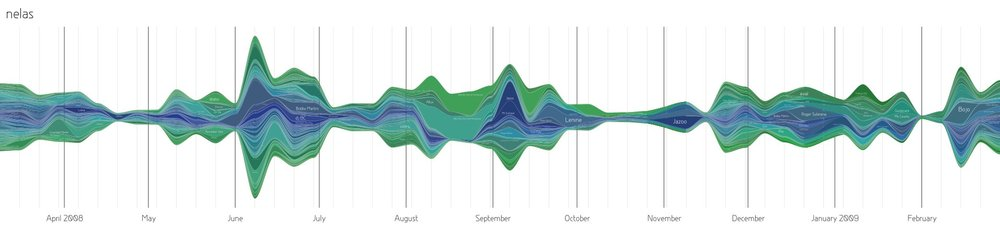
\includegraphics[width=\textwidth]{lastgraph}
    \caption[Figura simples]{Figura abstrata simples com largura igual à largura do texto.}
    \label{fig:last}
\end{figure}

\begin{figure}[htbp]
    \centering
    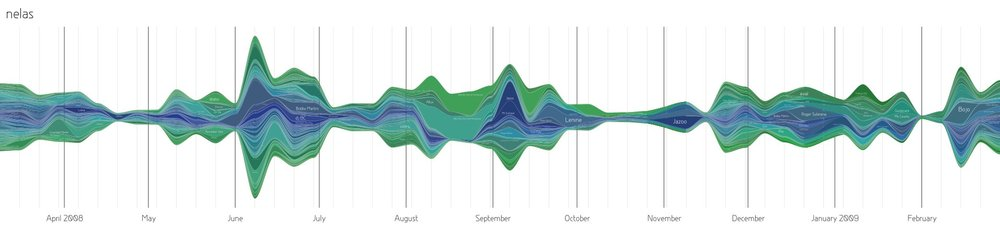
\includegraphics[width=0.5\textwidth]{lastgraph}
    \caption[Outra figura simples]{Figura abstrata simples com largura igual à metade da largura do texto.}
    \label{fig:last2}
\end{figure}

\subsection{Figuras compostas e abreviações}\label{cap2:res:figs2}

Você também pode inserir múltiplas figuras em uma só, permitindo alinhá-las de forma flexível e consistente (ver Figura~\ref{fig:fsm}).

% Usando o pacote nomencl
% Detalhe importante, leia as instruções no site para fazer a lista de abreviações aparecer.
% http://code.google.com/p/mestre-em-latex/wiki/ListaDeAbreviaturas
Para selecionar abreviações que serão incluídas na lista no começo do documento veja o arquivo \texttt{cap2.tex}; como a seguir as células mesenquimais primárias (CMP) iniciam sua ingressão.%
\nomenclature{CMP}{células mesenquimais primárias}

% Note como incluir as sublegendas para cada subfigura (subfloat) e como citá-las na legenda usando o comando subref.
% Note também como incluir as referências às abreviações (nomenclature) utilizadas para que sejam listadas no preâmbulo.
\begin{figure}[htbp]
    \centering
    \subfloat[Subfigura1]{\label{fig:t1}
\includegraphics[width=200pt]{fsm}}\vspace{11pt}
    \subfloat[Subfigura2]{\label{fig:t2}
\includegraphics[width=200pt]{fsm}}\\
    \vspace{-18pt}
    \subfloat[Subfigura3]{\label{fig:t3}
\includegraphics[width=200pt]{fsm}}\vspace{11pt}
    \subfloat[Subfigura4]{\label{fig:t4}
\includegraphics[width=200pt]{fsm}}%
    \caption[Figura com subfiguras]{Exemplo de figura com subfiguras. \subref{fig:t1}~Subfigura1 (\textbf{og}) na lâmina. \subref{fig:t2}~Subfigura2 (\textbf{oppv}). \subref{fig:t3}~Subfigura3 aderida (\textbf{opv}). \subref{fig:t4}~Subfigura4. \textbf{sg}, seio genital; \textbf{ln}, lúmen.}%
    \nomenclature{og}{oogônia}%
    \nomenclature{oppv}{oócitos primários pré-vitelogênicos}%
    \nomenclature{opv}{oócitos primários vitelogênicos}%
    \nomenclature{sg}{seio genital}%
    \nomenclature{ln}{lúmen}
    \label{fig:fsm}
\end{figure}

\section{Discussão}\label{cap2:disc}

A evolução deste caráter pode ser vista de duas formas:

% Este é um dos modos de iniciar uma lista ordenada.
% Note que é possível inserir listas dentro de listas.
\begin{enumerate}
  \item{Condição inicial $\longrightarrow$ Condição final}\label{hipo:1}
    \begin{itemize}
      \item{Primeira consequência}
      \item{Segunda consequência}
    \end{itemize}
  \item{Outra condição inicial $\longrightarrow$ Condição intermediária $\longrightarrow$ Outra condição final}\label{hipo:2}
    \begin{itemize}
      \item{Consequência alternativa}
    \end{itemize}
\end{enumerate}

Você pode citar ítens assinalados, como a hipótese~\ref{hipo:1} e a alternativa~\ref{hipo:2}.
